\chapter{State Of The Art}
\label{chapter3_state_of_the_art}
\thispagestyle{empty}

\vspace{0.5cm}

The integration of RL and neural networks has a long history. Early 
RL literature \cite{rummery1994line, tesauro1995temporal, bertsekas1995neuro}
presents \textit{connectionist} approaches in conjunction with a variety
of RL algorithms, mostly using dense ANNs as approximators for the value 
functions from low-dimensional (or engineered) state spaces.
The recent and exciting achievements of DL, however, have caused a sort of RL 
renaissance, with DRL algorithms outperforming classic RL techinques on 
environments which were previously considered intractable. 
Much like the game of Chess was believed out of the reach of machines until 
IBM's Deep Blue computer \cite{campbell2002deep} won against world champion 
Garry Kasparov in 1997, DRL has paved the way to solve a wide spectrum of 
complex tasks which were previously considered a stronghold of humanity. 

In this chapter we present the most important and recent results of DRL research, 
as well as some work related to the method proposed in this thesis.

\section{Value-based Deep Reinforcement Learning} \label{SOA:value}
In 2015, Mnih et al.\ \cite{mnih2015human} introduced the \textit{deep 
Q-learning} (DQN\footnote{Acronym of \textit{Deep Q-Network.}}) algorithm which 
basically ignited the field of DRL.
The important contributions of DQN consisted in providing an end-to-end 
framework to train an agent on the \textit{Atari} environments starting from 
the pixel-level representation of the states, with a deep CNN (called 
\textit{deep Q-network}) used to estimate the $Q$ function and apply greedy 
control. The authors were able to reuse the same architecture to solve many 
different games without the need for \textit{hyperparameter tuning}, which 
proved the effectiveness of the method.
%
\begin{figure}[h]
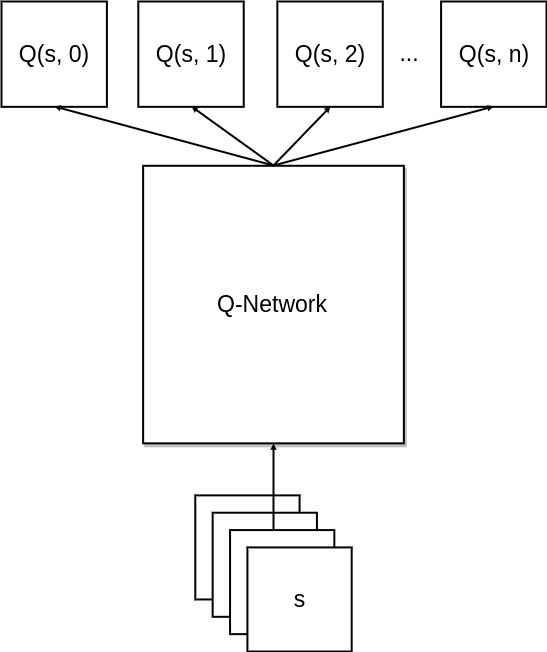
\includegraphics[width=0.5\textwidth]{pictures/dqn}
\centering
\caption{Structure of the Deep Q-Network by Mnih et al.\ }
\end{figure}
%

The key idea of DQN is to embed the update step of Q-learning into the loss used
for SGD to train the deep CNN, resulting in the following gradient update:
%
\begin{IEEEeqnarray}{rCl}
    %
    \frac{\partial L}{\partial W_i^{old}} = E[(r + \gamma \max_{a'} Q(s', a'; \theta') - Q(s, a)) \frac{\partial Q(s, a; \theta)}{\partial W_i^{old}}]
    %
\end{IEEEeqnarray}
%
where $\theta, \theta'$ indicate two different sets of parameters for the CNN, 
which are respectively called the \textit{online network} ($\theta$) to select 
the action for the collection of samples, and the \textit{target network} 
($\theta'$) to produce the update targets. The online network is continuously 
updated during training, whereas the target network is kept fixed for longer 
time intervals in order to stabilize the online estimate.
Moreover, a sampling procedure called \textit{experience replay} 
\cite{lin1992self} is used to stabilize training. This consists in keeping a
variable training set of transitions collected with increasingly better policies
(starting from a fully random $\varepsilon$-greedy policy and decreasing 
$\varepsilon$ as the $Q$ estimate improves), from which training samples are
randomly selected.
The full training procedure of DQN is reported in Algorithm \ref{alg:DQN}.
%
\begin{algorithm}[h]
    \caption{Deep Q-Learning with Experience Replay}
    \label{alg:DQN}
    \begin{algorithmic}
	\STATE Initialize replay memory $\mathcal{D}$ to capacity $N$
	\STATE Initialize action-value function $Q$ with two random sets of weights $\theta, \theta'$
	\FOR{$episode = 1,M$}
	    \FOR{$t = 1,T$}
		\STATE Select a random action $a_t$ with probability $\varepsilon$
		\STATE Otherwise, select $a_t = {\arg\max}_a Q(s_t, a; \theta)$
		\STATE Execute action $a_t$, collect reward $r_{t+1}$ and observe next state $s_{t+1}$
		\STATE Store the transition $(s_t, a_t, r_{t+1}, s_{t+1})$ in $\mathcal{D}$
		\STATE Sample minibatch of transitions $(s_j, a_j, r_{j+1}, s_{j+1})$ from $\mathcal{D}$
		\STATE Set $ y_j = \begin{cases} 
					r_{j+1}, & \mbox{if } s_{j+1}\mbox{ is terminal} \\ 
					r_{j+1} + \gamma \max_{a'} Q(s_{j+1}, a'; \theta'), & \mbox{otherwise}
				    \end{cases}$
		\STATE Perform a gradient descent step using targets $y_j$ with respect to the online parameters $\theta$
		\STATE Every $C$ steps, set $\theta' \leftarrow \theta$
	    \ENDFOR
	\ENDFOR
    \end{algorithmic}
\end{algorithm}
%
 
From this work (which we could call introductory), many improvements have been 
proposed in the literature.
%
\begin{figure}[h]
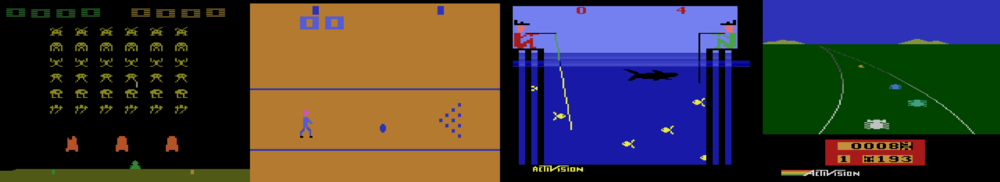
\includegraphics[width=\textwidth]{pictures/atari}
\centering
\caption{Some of the games available in the Atari environments}
\end{figure}
%
Van Hasselt et al.\ (2016) proposed \textit{Double DQN} (DDQN) \cite{van2016deep} 
to solve an over-estimation issue typical of Q-learning, due to the use of the 
maximum action value as an approximation for the maximum expected action value
(see Equation \eqref{eq:QL_update}).
This general issue was addressed by Van Hasselt (2010) with \textit{Double 
Q-learning} \cite{hasselt2010double}, a learning algorithm which keeps two 
separate estimates of the action-value function $Q^A$ and $Q^B$, and uses one to
update the other as follows:
%
\begin{IEEEeqnarray}{rCl}
    %
    Q^A(s, a) \leftarrow Q^A(s, a) + \alpha[r + \gamma Q^B(s', \underset{a}{\arg\max}Q^A(s', a)) - Q^A(s, a)]
    %
\end{IEEEeqnarray}
%
and vice-versa for $Q^B$.
DDQN uses a similar approach to limit over-estimation in DQN by evaluating the 
greedy policy according to the online network, but using the target network to 
estimate its value. This is achieved with a small change in the computation of 
the update targets:
%
\begin{IEEEeqnarray}{rCl}
    %
    y_j = \begin{cases} 
	    r_{j+1}, & \mbox{if } s_{j+1}\mbox{ is terminal} \\ 
		r_{j+1} + \gamma Q(s_{j+1}, \underset{a}{\arg\max}Q(s_{j+1}, a; \theta); \theta'), & \mbox{otherwise}
	  \end{cases}
    %
\end{IEEEeqnarray}
%    
DDQN performed better (higher median and mean score) on the 49 Atari games used 
as benchmark by Mnih et al.\ (2015), equaling or even surpassing humans on 
several games.

Schaul et al.\ (2016) \cite{schaul2016prioritized} developed the concept
of \textit{prioritized experience replay}, which replaced DQN's uniform sampling 
strategy from the replay memory with a sampling strategy weighted by the 
\textit{TD errors} committed by the network. This improved the performance of 
both DQN and DDQN.

Wang et al.\ (2016) introduced a slightly different end-to-end \textit{dueling 
architecture} \cite{wang2016dueling}, composed of two different deep estimators:
one for the state-value function $V$ and one for the \textit{advantage function} 
$A: S \times A \rightarrow \mathbb{R}$ defined as:
%
\begin{IEEEeqnarray}{rCl}
    %
    A^\pi(s, a) = Q^\pi(s, a) - V^\pi(s)
    %
\end{IEEEeqnarray}
%
In this approach, the two networks share the same convolutional layers
but use two separate dense layers. The two streams are then combined to estimate
the optimal action-value function as\footnote{In the original paper, the authors
explicitly indicate the dependence of the estimates on different 
parameters (e.g.\ $V^\pi(s, a; \phi, \alpha)$ where $\phi$ is the set of
parameters of the convolutional layers and $\alpha$ of the dense layers). 
For simplicity in the notation, here we report the estimates computed by the 
network with the same notation as the estimated functions (i.e.\ the network 
which approximates $V^\pi$ is indicated as $V^\pi$, and so on...).}:
%
    \begin{IEEEeqnarray}{rCl}
    %
    Q^\pi(s, a) = V^\pi(s) + (A^\pi(s, a) - \max_{a'}A^\pi(s, a'))
    %
    \end{IEEEeqnarray}
%
Several other extensions of the DQN algorithm have been proposed in recent years. 
Among these, we cite Osband et al.\ (2016) \cite{osband2016deep} who proposed 
a better exploration strategy based on Thompson sampling, to select an 
exploration policy based on the probability that it is the optimal policy; He et
al.\ (2017) \cite{he2017learning} added a constrained optimization approach 
called \textit{optimality tightening} to propagate the reward faster during 
updates and improve accuracy and convergence; Anschel et al.\ (2017) 
\cite{anschelaveraged} improved the variance and instability of DQN by averaging
previous $Q$ estimates; Munos et al.\ (2016) \cite{munos2016safe} and 
Harutyunyan et al.\ (2016) \cite{harutyunyan2016q} proposed to incorporate 
on-policy samples to the Q-learning target and seamlessly switch between 
off-policy and on-policy samples, which again resulted in faster reward 
propagation and convergence. 


\section{Other approaches}
\subsection{Memory architectures}
Graves et al.\ (2016) \cite{graves2016hybrid} proposed \textit{Differentiable 
Neural Computer} (DNC), an architecture in which an ANN has access to an 
external memory structure, and learns to read and write data by gradient descent
in a goal-oriented manner.
This approach outperformed normal ANNs and DNC's precursor \textit{Neural 
Turing Machine} \cite{gravesneural} on a variety of query-answering and natural 
language processing tasks, and was used to solve a simple \textit{moving block} 
puzzle with a form of reinforcement learning in which a sequence of instructions
describing a goal is coupled to a reward function that evaluates whether the 
goal is satisfied (a set-up that resembles an animal training protocol with a 
symbolic task cue).
%
\begin{figure}[h]
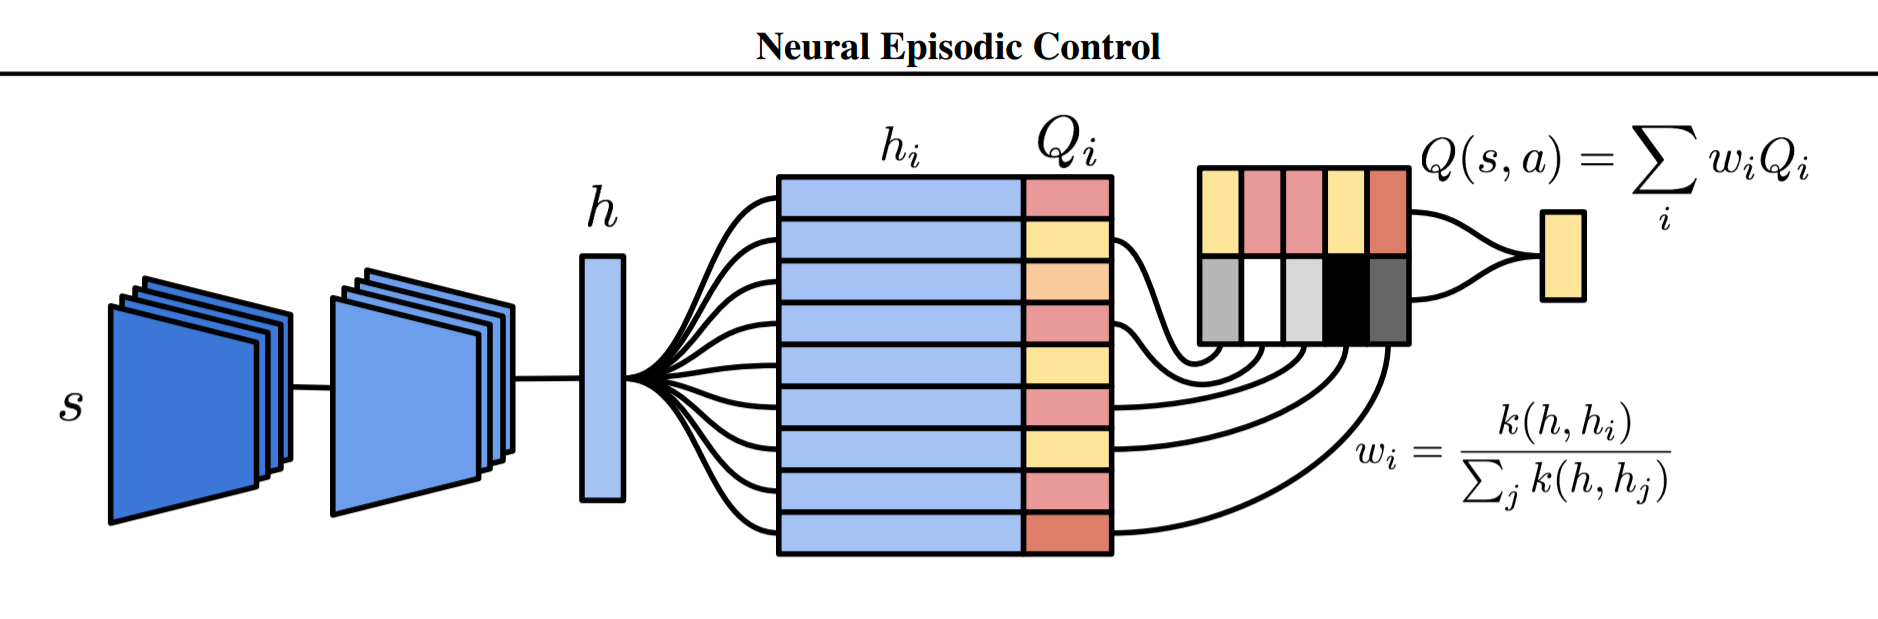
\includegraphics[width=\textwidth]{pictures/nec}
\centering
\caption[Architecture of NEC]{Architecture of NEC (image taken from 
			      \cite{pritzel2017neural})}
\label{f:nec}
\end{figure}
%

Pritzel et al.\ (2017) \cite{pritzel2017neural} extended the concept of 
differentiable memory to DQN with \textit{Neural Episodic Control} (NEC). 
In this apporach, the DRL agent consists of three components: a CNN which 
processes pixel images, a set of memory modules (one per action), and a dense 
ANN which converts read-outs from the action memories into action-values. The 
memory modules, called \textit{differentiable neural dictionaries} (DNDs), are 
memory structures which resemble the dictionary data type found in computer 
programs. DNDs are used in NEC to associate the state embeddings computed by the
CNN to a corresponding $Q$ estimate, for each visited state: a read-out for a 
key consists in a weighted sum of the values in the DND, with weights given by 
normalized kernels between the lookup key and the corresponding key in memory 
(see Figure \ref{f:nec}). 
DNDs are populated automatically by the algorithm without learning what to write,
which greatly speeds up the training time with respect to DNC.

NEC outperformed every previous DRL approach on Atari games, by achieving better
results using less training samples.

\subsection{AlphaGo}
Traditional board games like chess, checkers, Othello and Go are classical 
test benches for artificial intelligence. Since the set of rules which
characterizes this type of games is fairly simple to represent in a program, the
difficulty in solving these environments stems from the complexity of the 
state space. Among the cited games, Go was one of the last board games in which 
an algorithm had never beaten top human players, because its characteristic 
$19 \times 19$ board which allows for approximately $250^{150}$ sequences of
moves\footnote{Number of legal moves per position elevated to the length of the 
game.} was too complex for exhaustive search methods.
%
\begin{figure}[h]
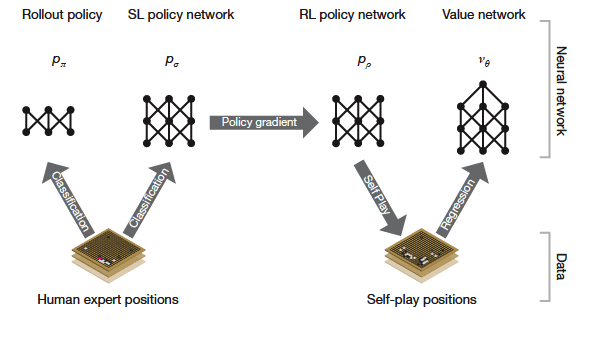
\includegraphics[width=\textwidth]{pictures/alphago}
\centering
\caption[Neural network training pipeline of AlphaGo]{Neural network training 
						      pipeline of AlphaGo
						      (image taken from 
						      \cite{silver2016mastering})}
\label{f:alphago}
\end{figure}
%

Silver et al.\ (2016) \cite{silver2016mastering} introduced \textit{AlphaGo}, 
a computer program based on DRL which won 5 games to 0 against the European Go 
champion in October 2015; soon after that, AlphaGo defeated 18-time world 
champion Lee Sedol 4 games to 1 in March 2016, and world champion Ke Jie 3 to 0 
in May 2017. After these results, Google DeepMind (the company behind 
AlphaGo) decided to retire the program from official competitions and released a
dataset containing 50 self-play games \cite{alphago}.

AlphaGo is a complex architecture which combines deep CNNs, reinforcement 
learning, and Monte Carlo Tree Search (MCTS) \cite{browne2012survey, gelly2012grand}. 
The process is divided in two phases: a neural network training pipeline and 
MCTS. In the training pipeline, four different networks are trained: a 
\textit{supervised learning} (SL) policy network trained to predict human moves;
a \textit{fast} policy network to rapidly sample actions during MC rollouts; a 
\textit{reinforcement learning} policy network that improves the SL network by 
optimizing the final outcome of games of self-play; a \textit{value} network 
that predicts the winner of games (see Figure \ref{f:alphago}). 
Finally, the policy and value networks are combined in an MCTS algorithm that 
selects actions with a lookahead search, by building a partial search tree using
the estimates computed with each network.

\subsection{Asynchronous Advantage Actor-Critic}
\textit{Actor-critic} algorithms \cite{sutton1998reinforcement} are TD methods 
that have a separate memory structure to explicitly represent the policy 
independent of the value function. The policy structure is known as the actor, 
because it is used to select actions, and the estimated value function is known 
as the critic, because it criticizes the actions made by the actor.
%
\begin{figure}[h]
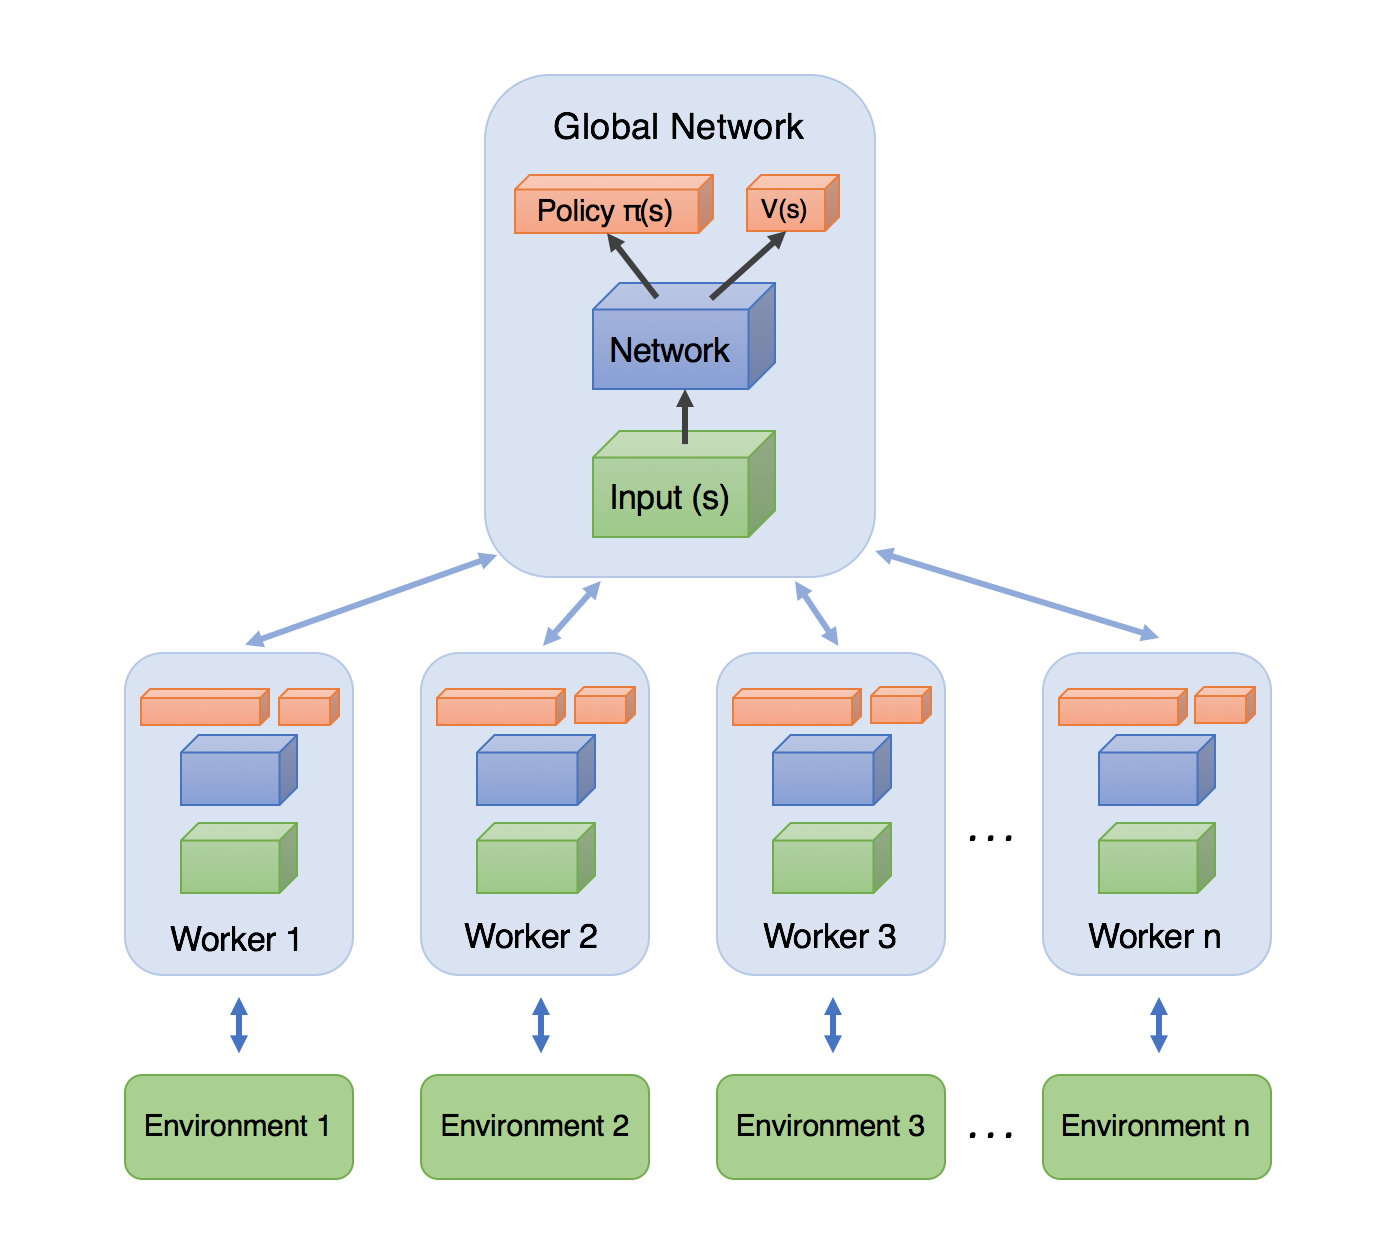
\includegraphics[width=\textwidth]{pictures/a3c}
\centering
\caption{The asynchronous architecture of A3C}
\label{f:a3c}
\end{figure}
%
Mnih et al.\ (2016) \cite{mnih2016asynchronous} presented a deep variation of 
the actor-critic algorithm, called \textit{Asynchronous Advantage Actor-Critic} 
(A3C). In this approach, different instances of actor-critic pairs are run in 
parallel (Figure \ref{f:a3c}) to obtain a lower-variance estimate of the value 
function, without the need of a replay memory to stabilize training. 
Each \textit{worker} consists in a deep CNN with a unique convolutional section 
and two separate dense networks on top, one for the value function and one for 
the policy. 

This asynchronous methodology was applied to other classical RL algorithms in 
the same paper; we only report the actor-critic variant as it was the best 
performing, with notably shorter training times and performance comparable 
to DQN and its variations.

\section{Related Work}
Lange and Riedmiller (2010) \cite{lange2010deep} proposed the \textit{Deep 
Fitted Q-iteration} (DFQ) algorithm, a batch RL method which used deep dense 
autoencoders to extract a state representation from pixel images. 
In this algorithm, a training set of $(s, a, r, s')$ transitions is collected
with a random exploration strategy, where $s, s'$ are pixel images of two 
consecutive states. The samples are then used to train a dense autoencoder with 
two neurons in the innermost layer, which in turn is used to encode all states 
in the training set. This encoded dataset is then passed as input to FQI, 
which produces an estimate for the $Q$ function using a kernel based 
approximator. A new policy is then computed from the estimated $Q$ and the 
encoder, and the process is repeated starting with the new policy until the 
obtained $Q$ is considered satisfactory.
The authors applied DFQ to a simple \textit{Gridworld} environment with fixed 
size and goal state, and were able to outperform other image-based feature
extraction methods (like \textit{Principal Components Analysis} 
\cite{wold1987principal}) with good sample efficiency.

% Another work which has common aspects with our method is the one by Anderson et
% al.\ (2015) \cite{anderson2015faster}, who improved convergence of DRL on 
% simple problems (e.g.\ \textit{Cart-pole} and \textit{Dynamic cart}) by 
% pre-training the Q-network to predict state dynamics.


























